\newcommand*{\includesDirectory}{includes}
\newcommand*{\settingsDirectory}{\includesDirectory/settings}
\newcommand*{\tikzDirectory}{\includesDirectory/tikz}

\documentclass[a4paper,12pt,oneside]{book}
\usepackage{geometry}
\usepackage{indentfirst}

\geometry{
    left=35mm,
    right=25mm,
    top=25mm,
    bottom=25mm
}

\renewcommand{\baselinestretch}{1.5}
\include{\settingsDirectory/language}
\usepackage{fancyhdr}
\pagestyle{fancy}
\fancyhf{}
\renewcommand{\headrulewidth}{0pt}
\fancyhead[R]{\thepage}

\fancypagestyle{plain}{
    \fancyhf{}
    \renewcommand{\headrulewidth}{0pt}
    \fancyhead[R]{\thepage}
}
\usepackage{titletoc}
\usepackage{hyperref}
\setcounter{tocdepth}{1}

\renewcommand\thechapter{Rozdział \Roman{chapter}}
\renewcommand\thesection{\arabic{section}.}
\renewcommand\thesubsection{\arabic{section}.\arabic{subsection}}
\contentsmargin{0.5cm}
\titlecontents{chapter}
    [2.2cm] %5.3
    {\vspace{0.2cm}}
    {\contentslabel[\thecontentslabel]{2.2cm}}%\thecontentslabel
    {\hspace*{-2.2cm}}% unnumbered chapters
    {\titlerule*[1cm]{.}\contentspage}[\vspace{0.2cm}]%

\titlecontents{section}
    [2.2cm] %5.3
    {}
    {\contentslabel[\thecontentslabel]{0.5cm}}
    {}
    {\titlerule*[0.5cm]{.}\contentspage}[]



\titlecontents{subsection}
    [2.8cm] %5.3
    {}
    {\contentslabel[\thecontentslabel]{0.7cm}}
    {}
    {\titlerule*[0.5cm]{.}\contentspage}[]



\usepackage{titlesec}


\titleformat{\chapter}[block]
  {\normalfont\huge}{\thechapter\vspace{-13pt}\\}{0pt}{\LARGE}
\titlespacing*{\chapter}{0pt}{0pt}{0pt}

\titleformat{\section}[block]
  {\normalfont}
  {\makebox[0.5cm][l]{\thesection}}{10pt}{}
\titlespacing*{\section}{0pt}{0pt}{0pt}

\titleformat{\subsection}[block]
  {\normalfont}
  {\hspace{1cm}\makebox[0.5cm][l]{\thesubsection}}{10pt}{}
\titlespacing*{\subsection}{0pt}{0pt}{0pt}
\usepackage{tikz}
\usepackage{tzplot}
\usetikzlibrary{shapes,quotes,angles,calc}

\tikzset {
    point/.style args = {reference: #1 x: #2 y: #3 label: #4 color: #5}{
        insert path = {
            \pgfextra{
                \node
                	[
                		circle,
                		fill = #5,
                		minimum size = 1 cm,
                		label = {\small{#4}},
                		scale = 0.13
                	]
                	at (#2,#3)
                	(#1) 
                	{};
            }
        }
    }
}
\tikzset {
    pointAndLabel/.style args = {reference: #1 x: #2 y: #3}{
        insert path = {
            \pgfextra{
                \path[point = reference: #1 x: #2 y: #3 label: $#1$ color: black];
            }
        }
    }
}

\begin{document}
    \thispagestyle{empty}
    \begin{center}
        \Huge{Otoczki wypukłe}
    \end{center}
    \tableofcontents	

  
    \chapterwithout{Wstęp}        

    \chapter{Omówienie teoretyczne otoczki wypukłej na płaszczyźnie}
    Otoczka wypukła zbioru punktów w swojej najbardziej podstawowej postaci jest wielokątem wypukłym obejmującym cały wszystkie punkty ze zbioru punktów leżących na płaszczyźnie w taki sposób aby wielokąt ten miał jak najmniejsze pole.    
    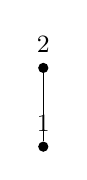
\begin{tikzpicture}
    \coordinate (a) at (0,0);
    \path[pointAndLabel = 
    	reference: 1 
    	x: 0
    	y: 0
	];
	\path[pointAndLabel = 
    	reference: 2
    	x: 0
    	y: 1
	];
	\draw (1)--
		  (2);
    \end{tikzpicture}      
    
    Dobrą reprezentacją otoczki wypukłej w świecie fizycznym może być grupa gwoździ przybita do płaskiej powierzchni i następnie opleciona ciasno sznurkiem. Gwoździe stykające się ze sznurkiem stanowiły będą wierzchołki otoczki wypukłej tej grupy gwoździ.
        \section{Otoczka wypukła zbioru punktów}
        W celu wyznaczenia otoczki wypukłej dla najbardziej ogólnego przypadku - nieuporządkowanego zbioru punktów na płaszczyźnie, możemy wykorzystać dwa najbardziej popularne algorytmy Algorytm Jarvisa oraz Algorytm Grahama.
        \subsection{Algorytm Grahama}
        
        \section{Otoczka wypukła wielokąta prostego}
        \section{Redukcja zbioru punktów do wielokąta prostego}
    \chapter{Zastosowania} 
    Istotnym, jeśli nie najistotniejszym zagadnieniem dotyczącym otoczek wypukłych są ich zastosowania. Już od kilkudziesięciu lat problem ten temat znajduje swoje użycie we wielu dziedzinach kombinatoryki i informatyki. Dla przykładu problem sortowania elementów liczbowych listy można sprowadzić do problemu znalezienia otoczki wypukłej. W związku z czym rozwiązanie tego problemu może pomóc w rozwiązaniu innych problemów w bardziej symboliczny i graficzny sposób.
        \section{Generalizacja kartograficzna}
        W celu jak najbardziej informatywnego i niezłożonego przedstawienia danych geograficznych w sposób graficzny potrzebne jest zastosowanie algorytmu generalizującego informacje.
		\section{Grafika komputerowa}
		Obiekty wykorzystywane w grafice komputerowej często mogą charakteryzować się skomplikowanymi kształtami. Im bardziej skomplikowany kształt tym więcej mocy obliczeniowej potrzebne będzie w celu wykonania danej operacji na tym kształcie. W niektórych przypadkach do uproszczenia graficznego danego obiektu używa się otoczki wypukłej jego kształtu. Ze względu na fakt, iż otoczka wypukła wielokąta zawsze będzie miała liczbę wierzchołków mniejszą lub równą liczbie wierzchołków samego wielokąta, powstała otoczka może posłużyć do wykonania mniejszej liczby obliczeń przy wykonywaniu operacji na danym obiekcie.
		\section{Detekcja obiektów}
        \section{Wyznaczanie obwiedni sygnału}
        
    \chapter{Dynamiczna otoczka wypukła}
    	\section{Algorytm}
    	\section{Implementacja w języku Scala} 
	\chapter{Podsumowanie} 
      
    \begin{thebibliography}{9}
    \addcontentsline{toc}{chapter}{Bibliografia}
    \bibitem{convexhullsimplepolygon}
    \href{https://mathweb.ucsd.edu/~ronspubs/83_09_convex_hull.pdf}
    {Ronald L. Graham, Frances Yao, Finding the Convex Hull of a Simple Polygon (1981)}
    \bibitem{online}
    \href{https://www.ime.usp.br/~walterfm/cursos/mac0331/2006/melkman.pdf}
    {Avraham A. Melkman, On-line Construction of the Convex Hull of a Simple Polyline (1985)}
    \bibitem{cartography}
    \href{https://www.isprs.org/proceedings/xxxiii/congress/part4/417_XXXIII-part4.pdf}
    {Jacqueleen Jourban, Yair Gabay, A Method for Construction of 2D Hull For Generalized Cartographic Representation (2000)}
    \bibitem{gpu}
    \href{https://www.sciencedirect.com/science/article/pii/S0097849312000544}
    {Min Tang, Jie-yi Zhao, Ruo-feng Tong, Dinesh Manocha, GPU accelerated convex hull computation (2012)}
    \bibitem{detection}
     \href{https://www.sciencedirect.com/science/article/pii/S1051200416300318}
     {Navjot Singh, Rinki Arya, R.K. Agrawal, A convex hull approach in conjunction with Gaussian mixture model for salient object detection (2016)}
    \bibitem{dynamic}
    \href{https://www.sciencedirect.com/science/article/pii/S1568494619306775}
    {Fan Cheng, Qiangqiang Zhang, Ye Tian, Xingyi Zhang, Maximizing receiver operating characteristics convex hull via dynamic reference point-based multi-objective evolutionary algorithm (2019)}
\end{thebibliography}
\end{document}
